\documentclass[a4paper,12pt]{article}
\usepackage{graphicx} % Required for inserting images
\usepackage[utf8]{vietnam}
\usepackage{amssymb}
\usepackage{amsmath}
\usepackage{amsfonts}
\usepackage{subfigure}


\pagenumbering{arabic}

\begin{document}

\begin{titlepage}
    \begin{center}
        \textbf{\large ĐẠI HỌC BÁCH KHOA HÀ NỘI}\\
        \textbf{\large Trường Công nghệ Thông tin và Truyền thông}\\[1cm]
        \includegraphics[width=100pt]{logo.png} \\[3cm] % Thay đường dẫn bằng đường dẫn tới logo của trường
       
        
        \textbf{\Huge BÁO CÁO BÀI TẬP CUỐI KỲ 2023.2}\\[0.5cm]
        \textbf{\Huge Học phần: Thực hành cơ sở dữ liệu}\\[0.5cm]
        \textbf{\Huge Mã học phần: IT3290}\\[0.5cm]
        \textbf{Giảng viên hướng dẫn:} Lê Đức Hậu\\
        \begin{flushleft}
            \textbf{Họ và tên:} Võ Anh Khôi\\[0.5cm]
            \textbf{Mã sinh viên:} [Mã Sinh Viên]\\[0.5cm]
        
        \end{flushleft}
        
        \vfill
        
        \textbf{\large Hà Nội, ngày [Ngày] tháng [Tháng] năm [Năm]}
        
    \end{center}
\end{titlepage}

\section{Mô tả bài toán}
\begin{itemize}
    \item Một trường đại học có một hệ thống ký túc xá lớn với nhiều tòa nhà và phòng khác nhau. Trường muốn xây dựng một hệ thống quản lý ký túc xá để dễ dàng theo dõi và quản lý các thông tin liên quan đến sinh viên, phòng ở, và các dịch vụ liên quan.
    \item Yêu cầu hệ thống
    \begin{enumerate}
        \item Quản lý sinh viên
        \item Quản lý thông tin phòng
        \item Quản lý thông tin trang thiết bị
        \item Quản lý dịch vụ và tiện ích
        \item Quản lý thành toán
        \item Quản lý bảo trì và sự cố
    \end{enumerate}
    \item Các chức năng chính của hệ thống
    \begin{enumerate}
        \item Đăng ký và quản lý thông tin sinh viên
        \item Quản lý phòng ở, trang thiết bị
        \item Quản lý dịch vụ và tiện ích
        \item Quản lý thanh toán
        \item Quản lý bảo trì và sự cố
    \end{enumerate}
\end{itemize}
\newpage
\section{Mô Hình thực thể liên kết}
\begin{figure}[tbh]
    \centering
    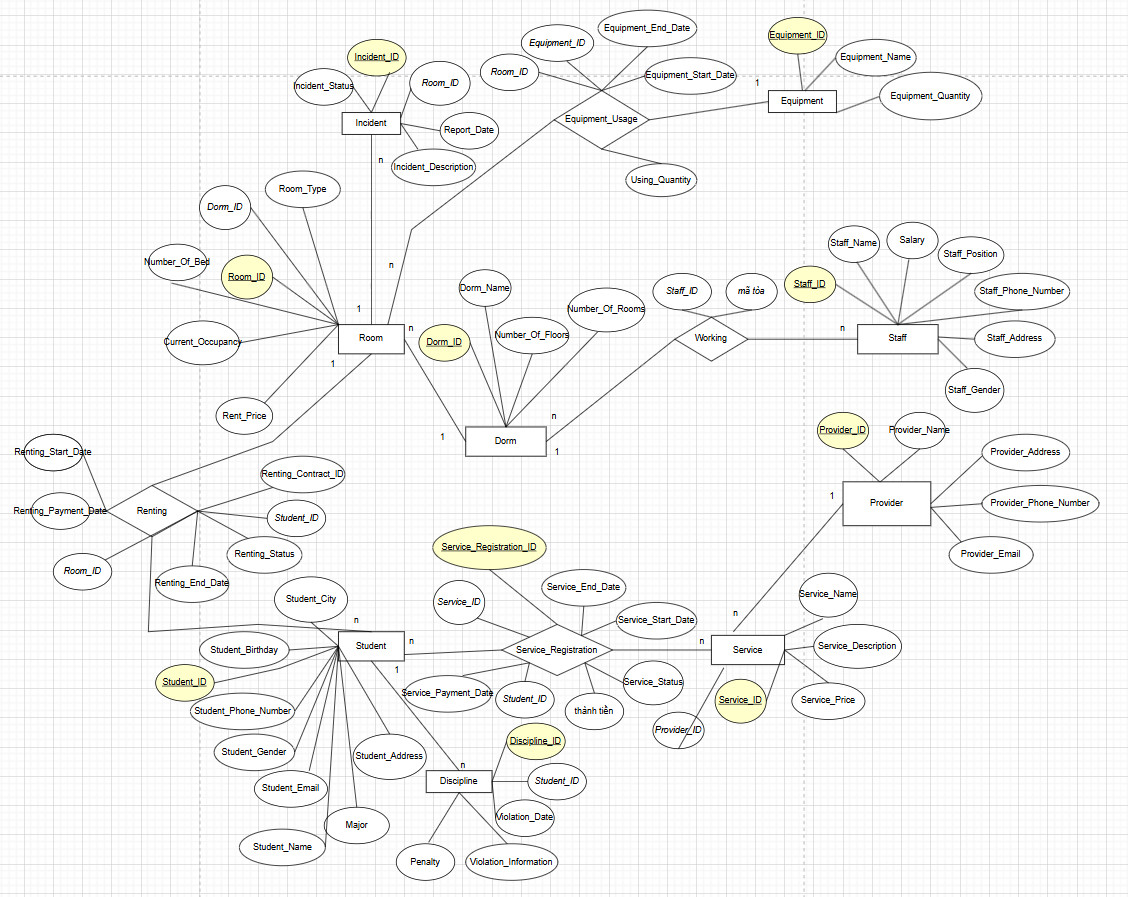
\includegraphics[width=0.8\textwidth]{ERD.jpg} % Thay 'path/to/your/image.jpg' bằng đường dẫn đến ảnh của bạn
    \caption{Mô hình ERD}
    \label{ERD}
\end{figure}

\section{Mô hình quan hệ}
\begin{figure}[tbh]
    \centering
    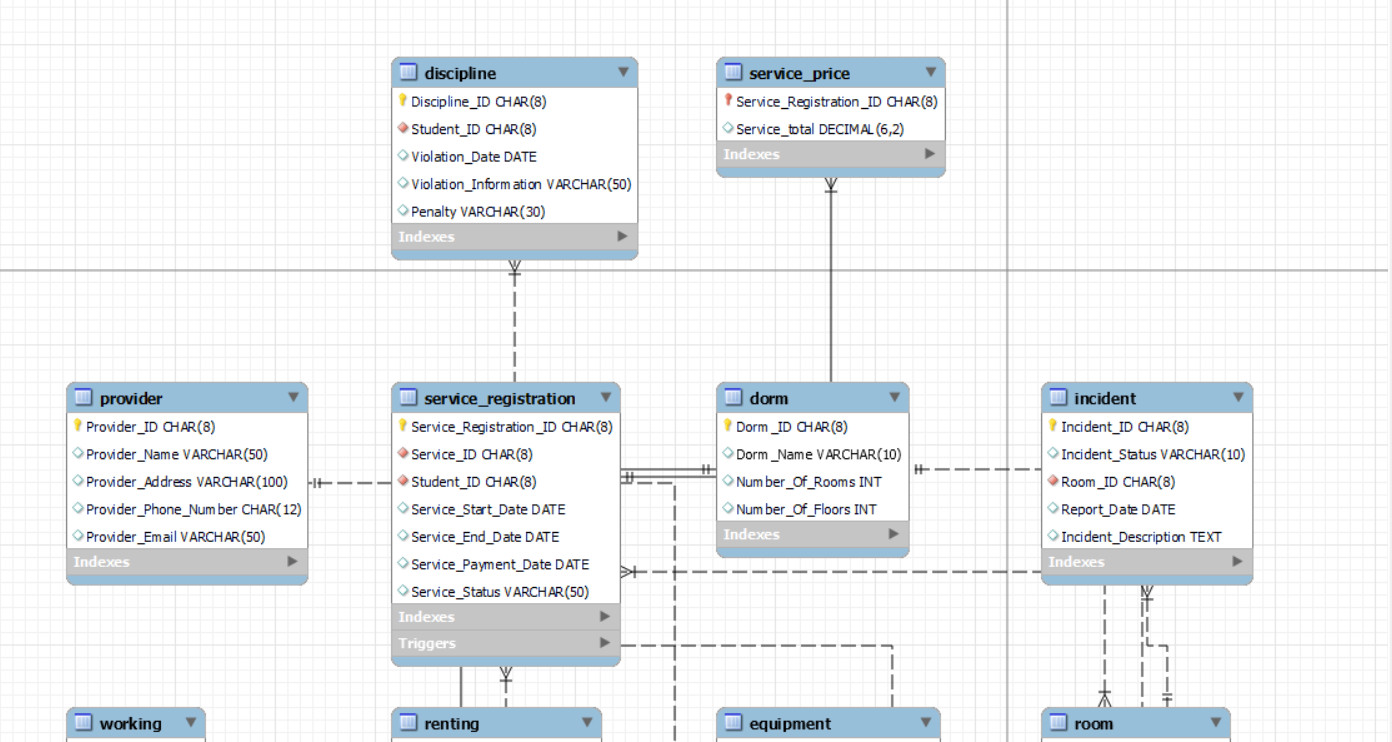
\includegraphics[width=0.8\textwidth]{ER1.jpg} 
\\ [1cm]
    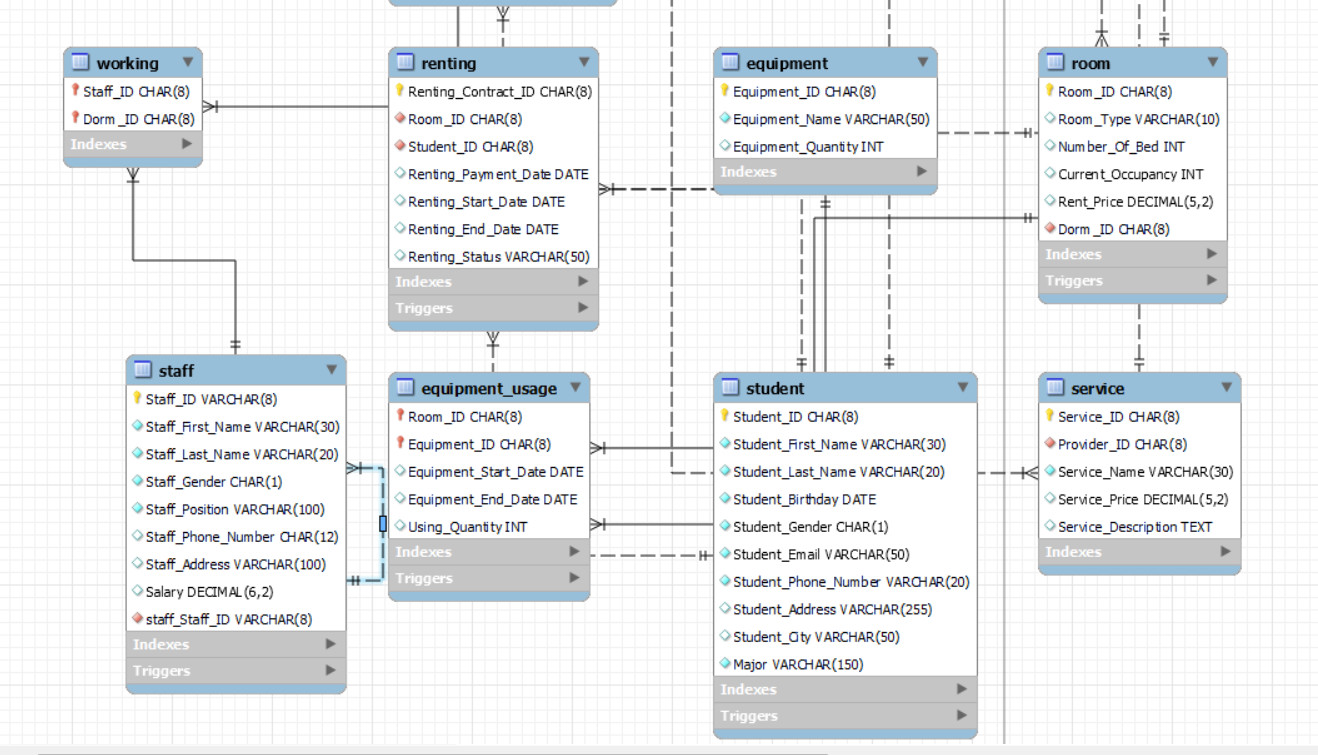
\includegraphics[width=0.8\textwidth]{ER2.jpg}
    \caption{Mô hình Quan hệ}
    \label{ERD}
\end{figure}
\newpage
\section{Trigger và Role}
\subsection{Trigger}
\begin{enumerate}
    \item \begin{verbatim}
Kiểm tra xem việc điền giới tính có hợp lệ không trước khi insert vào student
    DELIMITER $$

CREATE TRIGGER check_student_gender_before_insert
BEFORE INSERT ON Student
FOR EACH ROW
BEGIN
    -- Check if the gender is valid
    IF NEW.Student_Gender NOT IN ('M', 'F') THEN
        SIGNAL SQLSTATE '45000'
        SET MESSAGE_TEXT = 'Invalid gender. Must be M or F';
    END IF;
END$$

    DELIMITER ;
    \end{verbatim}
    \item \begin{verbatim}
Kiểm tra xem việc điền giới tính có hợp lệ không trước khi insert vào student
    DELIMITER $$

CREATE TRIGGER check_staff_gender_before_insert
BEFORE INSERT ON Staff
FOR EACH ROW
BEGIN
    -- Check if the gender is valid
    IF NEW.Staff_Gender NOT IN ('M', 'F') THEN
        SIGNAL SQLSTATE '45000'
        SET MESSAGE_TEXT = 'Invalid gender. Must be M or F';
    END IF;
END$$

    DELIMITER ;

    \end{verbatim}
    \item \begin{verbatim}
Kiểm tra xem phòng có đầy không trước khi insert
    DELIMITER $$

CREATE TRIGGER check_occupancy_before_insert
BEFORE INSERT ON Room
FOR EACH ROW
BEGIN
    IF NEW.Current_Occupancy > NEW.Number_Of_Bed THEN
        SIGNAL SQLSTATE '45000' SET MESSAGE_TEXT = 'Current occupancy cannot be greater than the number of beds';
    END IF;
END $$

CREATE TRIGGER check_occupancy_before_update
BEFORE UPDATE ON Room
FOR EACH ROW
BEGIN
    IF NEW.Current_Occupancy > NEW.Number_Of_Bed THEN
        SIGNAL SQLSTATE '45000' SET MESSAGE_TEXT = 'Current occupancy cannot be greater than the number of beds';
    END IF;
END $$

    DELIMITER ;
    \end{verbatim}
    \item \begin{verbatim}
+1 vào occupancy khi 1 sinh viên thuê thêm phòng
    DELIMITER $$
CREATE TRIGGER update_occupancy_on_renting
AFTER INSERT ON Renting
FOR EACH ROW
BEGIN
  DECLARE available_beds INT;
  DECLARE End_Date Date;

  SELECT Number_Of_Bed - Current_Occupancy INTO available_beds
  FROM Room
  WHERE Room.Room_ID = NEW.Room_ID;
  
  SELECT Renting_End_Date INTO End_Date
	FROM Renting
  WHERE Renting.Room_ID = NEW.Room_ID AND Renting.Student_ID = NEW.Student_ID ;
  IF available_beds > 0  THEN
	IF NOW() < End_Date THEN
    -- Cập nhật Current_Occupancy
    UPDATE Room
    SET Current_Occupancy = Current_Occupancy + 1
    WHERE Room.Room_ID = NEW.Room_ID;
    END IF;
  ELSE
    SIGNAL SQLSTATE '45000' SET MESSAGE_TEXT = 'Cannot rent room, maximum capacity reached.';
  END IF;
END; $$
    DELIMITER ;
    \end{verbatim}
    \item \begin{verbatim}
Kiểm tra xem giới tính sinh viên có phù hợp với phòng thuê hay không
    DELIMITER $$

CREATE TRIGGER Renting_Gender_check
BEFORE INSERT ON Renting
FOR EACH ROW
BEGIN
  DECLARE room_type VARCHAR(10);
  DECLARE student_gender CHAR(1);

  -- Lấy giới tính của sinh viên từ bảng Student
  SELECT Student.Student_Gender INTO student_gender
  FROM Student
  WHERE Student.Student_ID = NEW.Student_ID;

  -- Lấy loại phòng từ bảng Room
  SELECT Room.Room_Type INTO room_type
  FROM Room
  WHERE Room.Room_ID = NEW.Room_ID;

  -- So sánh giới tính và loại phòng
  IF (room_type = 'Female' AND student_gender <> 'F') OR (room_type = 'Male' AND student_gender <> 'M') THEN
    SIGNAL SQLSTATE '45000'
    SET MESSAGE_TEXT = 'Giới tính của sinh viên không phù hợp với loại phòng.';
  END IF;
END$$

    DELIMITER ;
    \end{verbatim}
    \item \begin{verbatim}
Tính toán thành tiền dịch vụ phải trả
    DELIMITER $$

CREATE TRIGGER Calculate_Total_Amount_Monthly
AFTER INSERT ON Service_Registration
FOR EACH ROW
BEGIN
  DECLARE total_amount DECIMAL(10, 2);
  DECLARE service_month INT;  -- Use INT for whole months
  DECLARE month_service_price DECIMAL(10,2);

  SELECT Service.Service_Price INTO month_service_price
  FROM Service
  WHERE Service.Service_ID = NEW.Service_ID;

  SET service_month = CEIL(DATEDIFF(NEW.Service_End_Date,NEW.Service_Start_Date) / 30.44);

  SET total_amount = service_month * month_service_price;

 INSERT INTO Service_Price 
  SET Service_Price.Service_total = total_amount,
		Service_Price.Service_Registration_ID = NEW.Service_Registration_ID;
END $$

DELIMITER ;
    \end{verbatim}
    \item \begin{verbatim}
Kiểm tra xem số thiết bị còn lại có đủ để mượn không
    DELIMITER $$
CREATE TRIGGER trg_check_equipment_usage
BEFORE INSERT ON Equipment_Usage
FOR EACH ROW
BEGIN
    DECLARE use_quantity INT;
    DECLARE total_quantity INT;
    -- Tính tổng số lượng thiết bị đang sử dụng cho thiết bị cụ thể trong bảng Equipment_Usage
    SELECT SUM(Using_Quantity)
    INTO use_quantity
    FROM Equipment_Usage
    GROUP BY  Equipment_Usage.Equipment_ID
	HAVING Equipment_Usage.Equipment_ID = NEW.Equipment_ID;


    SELECT Equipment_Quantity
    INTO total_quantity
    FROM Equipment
    WHERE Equipment.Equipment_ID = NEW.Equipment_ID;

    -- Kiểm tra nếu số lượng thiết bị sử dụng cộng với số lượng mới chèn lớn hơn số lượng thiết bị hiện có
    IF use_quantity + NEW.Using_Quantity > total_quantity THEN
        SIGNAL SQLSTATE '45000'
        SET MESSAGE_TEXT = 'Số lượng thiết bị sử dụng vượt quá số lượng thiết bị hiện có';
    END IF;
END $$
    \end{verbatim}
\end{enumerate}

\subsection{Role}
\begin{verbatim}
    Các loại role hiện có:
    Dev: ALL
    manager: SELECT, UPDATE, DELETE, INSERT
    accountant:SELECT 
    register: SELECT, INSERT, UPDATE
    reception; SELECT  Dorm Room Renting Student

\end{verbatim}
\section{Các truy vấn}
\begin{enumerate}
    \item \begin{verbatim}
Xóa mọi thông tin liên quan đến sinh viên có ID nhập vào 
DELIMITER $$
CREATE PROCEDURE delete_student(
    IN student_id VARCHAR(10)
)
BEGIN
    START TRANSACTION;
    
    DELETE FROM Renting WHERE Student_ID = student_id;
    DELETE FROM Service_Registration WHERE Student_ID = student_id;
    DELETE FROM Student WHERE Student_ID = student_id;
    
    COMMIT;
END $$
    DELIMITER ;
\end{verbatim}
\item \begin{verbatim}
Truy vấn nhân viên theo mã tòa
DELIMITER $$
CREATE PROCEDURE get_staff_info(IN dorm_id VARCHAR(150))
BEGIN
    SELECT 
        Staff.Staff_ID, 
        Staff.Staff_First_Name, 
        Staff.Staff_Last_Name, 
        Working.Dorm_ID
    FROM  Staff
    JOIN   Working ON Staff.Staff_ID = Working.Staff_ID
    WHERE   Working.Dorm_ID = dorm_id
    ORDER BY  Working.Dorm_ID;
END $$
DELIMITER ;
\end{verbatim}
\item \begin{verbatim}
Sắp xếp các phòng theo số lượng người 
DELIMITER $$
CREATE PROCEDURE get_rooms_by_occupancy()
BEGIN
     SELECT * FROM Room ORDER BY Current_Occupancy DESC;
end $$
   DELIMITER;
\end{verbatim}
\item \begin{verbatim}
Thêm dịch vụ mới vào bảng Service
DELIMITER $$
CREATE PROCEDURE add_new_service(
    IN p_service_id VARCHAR(10),
    IN p_provider_id VARCHAR(10),
    IN p_service_name VARCHAR(50),
    IN p_service_price DECIMAL(10,2),
    IN p_service_description VARCHAR(200)
)
BEGIN
    INSERT INTO Service (
        Service_ID, 
        Provider_ID, 
        Service_Name, 
        Service_Price, 
        Service_Description
    )
    VALUES (
        p_service_id,
        p_provider_id, 
        p_service_name,
        p_service_price,
        p_service_description
    );
END $$
DELIMITER ;
\end{verbatim}
\item \begin{verbatim}
Hiển thị tất cả sinh viên theo giới tính
DELIMITER $$
CREATE PROCEDURE get_sexual_students(IN sexual VARCHAR (10))
BEGIN 
 SELECT * FROM Student WHERE Student.Gender = sexual ;
END $$
DELIMITER ;
\end{verbatim}
\item \begin{verbatim}
Tính toán tỷ lệ lấp đầy kí túc xá
DELIMITER $$
CREATE PROCEDURE get_dorm_occupancy_rates()
BEGIN
   SELECT Dorm.Dorm_Name,
       SUM(Room.Current_Occupancy) / SUM(Room.Number_Of_Bed) * 100 AS Occupancy_Rate
  FROM Dorm
  JOIN Room ON Dorm.Dorm_ID = Room.Dorm_ID
GROUP BY Dorm.Dorm_Name;
END $$
DELIMITER ;
\end{verbatim}
\item \begin{verbatim}
Hiển thị tất cả thông tin của 1 sinh viên 
DELIMITER $$
CREATE PROCEDURE get_student_by_name(
    IN first_name VARCHAR(50),
    IN last_name VARCHAR(50)
)
BEGIN
    SELECT * 
    FROM Student
    WHERE Student_First_Name = first_name AND Student_Last_Name = last_name;
END $$
DELIMITER ;
\end{verbatim}
\item \begin{verbatim}
 Kiểm tra các sự cố xảy ra vào ngày tháng nhập vào
DELIMITER $$
CREATE PROCEDURE get_incidents_by_month_year(
    IN report_year INT,
    IN report_month INT
)
BEGIN
    SELECT *
    FROM Incident
    WHERE YEAR(Incident.Report_Date) = report_year
      AND MONTH(Incident.Report_Date) = report_month;
END $$
DELIMITER ;
\end{verbatim}
\item \begin{verbatim}
Tăng lương cho 1 nhân viên cụ thể lên x lần
DELIMITER $$
CREATE PROCEDURE update_staff_salary(
    IN staff_id VARCHAR(20),
    IN salary_increase DECIMAL(10,2)
)
BEGIN
    UPDATE Staff
    SET Staff_Salary = Staff_Salary * (1 + salary_increase)
    WHERE Staff_ID = staff_id;
END $$
DELIMITER ;
\end{verbatim}
\item \begin{verbatim}
Thông tin chi tiết về các nhà cung cấp và dịch vụ của họ
DELIMITER $$
CREATE PROCEDURE get_provider_service_info()
BEGIN
    SELECT 
        Provider.Provider_Name,
        Provider.Provider_Address,
        Provider.Provider_Phone_Number,
        Service.Service_Name,
        Service.Service_Price
    FROM Provider
    JOIN Service ON Provider.Provider_ID = Service.Provider_ID;
END $$
DELIMITER ;
\end{verbatim}
\item \begin{verbatim}
Danh sách sinh viên chưa thanh toán tiền thuê phòng
DELIMITER $$
CREATE PROCEDURE get_unpaid_renting_contracts()
BEGIN
    SELECT 
        Student.Student_ID,
        Student.Student_First_Name,
        Student.Student_Last_Name,
        Renting.Renting_Contract_ID,
        Renting.Renting_Status
    FROM Student
    JOIN Renting ON Student.Student_ID = Renting.Student_ID
    WHERE Renting.Renting_Status = 'not paid';
END $$
DELIMITER ;
\end{verbatim}
\item \begin{verbatim}
Thông tin chi tiết về thiết bị trong từng ký túc xá
DELIMITER $$
CREATE PROCEDURE get_dorm_equipment_usage()
BEGIN
    SELECT 
        Dorm.Dorm_Name,
        Equipment.Equipment_Name,
        SUM(Equipment_Usage.Using_Quantity) AS Total_Quantity
    FROM Dorm
    JOIN Room ON Dorm.Dorm_ID = Room.Dorm_ID
    JOIN Equipment_Usage ON Room.Room_ID = Equipment_Usage.Room_ID
    JOIN Equipment ON Equipment_Usage.Equipment_ID = Equipment.Equipment_ID
    GROUP BY Dorm.Dorm_Name, Equipment.Equipment_Name;
END $$
DELIMITER ;
\end{verbatim}
\item \begin{verbatim}
Thông tin thiết bị trong từng phòng
DELIMITER $$
CREATE PROCEDURE get_room_equipment_usage()
BEGIN
    SELECT 
        Room.Room_ID,
        Room.Room_Type,
        Equipment.Equipment_Name,
        Equipment_Usage.Using_Quantity,
        Equipment_Usage.Equipment_Start_Date,
        Equipment_Usage.Equipment_End_Date
    FROM Room
    JOIN Equipment_Usage ON Room.Room_ID = Equipment_Usage.Room_ID
    JOIN Equipment ON Equipment_Usage.Equipment_ID = Equipment.Equipment_ID ORDER BY Room.Room_ID;
END $$
DELIMITER ;
\end{verbatim}
\item \begin{verbatim}
Thống kê số lượng sinh viên theo ngành học
DELIMITER $$
CREATE PROCEDURE get_student_major_counts()
BEGIN
    SELECT 
        Major,
        COUNT(Student_ID) AS Total_Students
    FROM Student
    GROUP BY Major
    ORDER BY Total_Students DESC;
END $$
DELIMITER ;
\end{verbatim}
\item \begin{verbatim}
Các phòng có số người ở tối đa và cần mở rộng
DELIMITER $$
CREATE PROCEDURE get_full_rooms()
BEGIN
    SELECT 
        Room.Room_ID,
        Room.Room_Type,
        Room.Number_Of_Bed,
        Room.Current_Occupancy
    FROM Room
    WHERE Room.Current_Occupancy = Room.Number_Of_Bed;
END $$
DELIMITER ;
\end{verbatim}
\item \begin{verbatim}
 Chi tiết lịch sử thuê phòng của từng sinh viên
DELIMITER $$
CREATE PROCEDURE get_student_renting_details()
BEGIN
    SELECT 
        Student.Student_ID,
        Student.Student_First_Name,
        Student.Student_Last_Name,
        Room.Room_ID,
        Room.Room_Type,
        Renting.Renting_Start_Date,
        Renting.Renting_End_Date,
        Renting.Renting_Status
    FROM Student
    JOIN Renting ON Student.Student_ID = Renting.Student_ID
    JOIN Room ON Renting.Room_ID = Room.Room_ID
    ORDER BY Student.Student_ID, Renting.Renting_Start_Date;
END $$
DELIMITER ;
\end{verbatim}
\item \begin{verbatim}
 Danh sách sinh viên có hợp đồng thuê sắp hết hạn trong tháng này
DELIMITER $$
CREATE PROCEDURE get_students_returning_equipment_this_month()
BEGIN
    SELECT 
        Student.Student_ID, 
        Student.Student_First_Name, 
        Student.Student_Last_Name,
        Renting.Renting_End_Date
    FROM Student
    JOIN Renting ON Student.Student_ID = Renting.Student_ID
    WHERE MONTH(Renting.Renting_End_Date) = MONTH(CURDATE()) 
        AND YEAR(Renting.Renting_End_Date) = YEAR(CURDATE());
END $$
DELIMITER ;
\end{verbatim}
\item \begin{verbatim}
Danh sách các sinh viên đã hoàn thành tất cả các khoản thanh toán
DELIMITER $$
CREATE PROCEDURE get_students_with_no_unpaid_items()
BEGIN
    SELECT 
        Student.Student_ID, 
        Student.Student_First_Name, 
        Student.Student_Last_Name
    FROM Student
    WHERE Student.Student_ID NOT IN (
        SELECT Student_ID
        FROM Renting
        WHERE Renting_Status = 'not paid'
    )
    AND Student.Student_ID NOT IN (
        SELECT Student_ID
        FROM Service_Registration
        WHERE Service_Status = 'not paid'
    );
END $$
DELIMITER ;
\end{verbatim}
\item \begin{verbatim}
hiện thông tin của tất cả sinh viên ở thành phố
DELIMITER $$
create procedure tt_sv1(thanh_pho varchar(150))
begin
   select Student_ID, Student_First_Name, Student_Last_Name, Student_Birthday, Student_Gender, Student_Email, Student_Phone_Number, Student_Address, Student_City, Major
   from student 
   where Student_City=thanh_pho;
   end $$
DELIMITER;
\end{verbatim}
\item \begin{verbatim}
hiện thông tin sinh viên có mã ngành học
DELIMITER $$
create procedure tt_sv(ma_ng varchar(150))
begin
   select Student_ID, Student_First_Name, Student_Last_Name, Student_Birthday, Student_Gender, Student_Email, Student_Phone_Number, Student_Address, Student_City, Major
   from student 
   where Major=ma_ng;
   end $$
   DELIMITER;
\end{verbatim}
\item \begin{verbatim}
hiện thông tin những sinh viên sinh năm được nhập
DELIMITER $$
create procedure tt_sv2(nam_sinh varchar(150))
begin
   select Student_ID, Student_First_Name, Student_Last_Name, Student_Birthday, Student_Gender, Student_Email, Student_Phone_Number, Student_Address, Student_City, Major
   from student 
   where year(Student_Birthday)=nam_sinh;
   end $$
   DELIMITER;
\end{verbatim}
\item \begin{verbatim}
thông tin những sinh viên ở mã phòng 
delimiter $$
create procedure tt_sv_maphong(id_p varchar(50))
begin
select Student_ID, Student_First_Name, Student_Last_Name, Student_Birthday, Student_Gender, Student_Email, Student_Phone_Number, Student_Address, Student_City, Major
from student
where 	Student_ID in
(select Student_ID
from renting
where Room_ID = id_p
);
end $$
delimiter;
\end{verbatim}
\item \begin{verbatim}
Danh sách sv đã đăng kí dịch vụ
delimiter $$
create procedure tt_sv_da_dkdv()
begin
select s.Student_ID, s.Student_First_Name, s.Student_Last_Name, s.Student_Birthday, s.Student_Gender, s.Student_Email, s.Student_Phone_Number, s.Student_Address, s.Student_City, s.Major
from student s
join service_registration on service_registration.Student_ID=s.Student_ID;
end $$
delimiter;
\end{verbatim}
\item \begin{verbatim}
Tổng số sv,nv,phòng cho mỗi ktx
 delimiter $$
create procedure tong_nv_sv_phong_moi_toa()
begin
SELECT d.Dorm_Name,
     (SELECT COUNT(*) FROM Student s JOIN Renting r ON s.Student_ID = r.Student_ID WHERE r.Room_ID IN (SELECT Room_ID FROM Room WHERE Dorm_ID = d.Dorm_ID)) AS Total_Students,
     (SELECT COUNT(*) FROM Room WHERE Dorm_ID = d.Dorm_ID) AS Total_Rooms,
     (SELECT COUNT(*) FROM Staff WHERE Dorm_ID = d.Dorm_ID) AS Total_Staff
FROM Dorm as d
LIMIT 0, 1000;
end $$
delimiter;
\end{verbatim}
\item \begin{verbatim}
những sinh viên vi phạm kỉ luật và thông tin hành vi của sv
delimiter $$
create procedure tt_sv_vp_ky_luat()
begin
SELECT s.Student_ID, s.Student_First_Name, s.Student_Last_Name, d.Violation_Date, d.Violation_Information, d.Penalty
FROM Student s
JOIN Discipline d ON s.Student_ID = d.Student_ID;
end $$
delimiter;
\end{verbatim}
\item \begin{verbatim}
Tổng doanh thu đăng kí dịch vụ của sv
delimiter $$
create procedure tong_doanh_thu_dk_dv_cua_sv()
begin
SELECT s.Student_ID, s.Student_First_Name, s.Student_Last_Name, SUM(sp.Service_total) AS Total_Service_Revenue
FROM Student s
JOIN Service_Registration sr ON s.Student_ID = sr.Student_ID
JOIN Service_price sp ON sr.Service_Registration_ID = sp.Service_Registration_ID
GROUP BY s.Student_ID, s.Student_First_Name, s.Student_Last_Name;
end $$
delimiter;
\end{verbatim}
\item \begin{verbatim}
Thông tin các phòng có sự cố và chi tiết sự cố
delimiter $$
create procedure tt_phong_co_su_co_va_chi_tiet_su_co()
begin
SELECT r.Room_ID, i.Incident_ID, i.Incident_Status, i.Report_Date, i.Incident_Description
FROM room r
JOIN incident i ON r.Room_ID = i.Room_ID;
end $$
delimiter;
\end{verbatim}
\item \begin{verbatim}
Thông tin dịch vụ đang dùng và tổng doanh thu dịch vụ tương ứng
delimiter $$
create procedure tt_dv_va_tong_doanh_thu_tuong_ung()
begin
SELECT p.Provider_Name,s.Service_Name,SUM(sp.Service_total) AS Total_Revenue
FROM provider p
JOIN service s ON p.Provider_ID = s.Provider_ID
LEFT JOIN service_registration sr ON s.Service_ID = sr.Service_ID
LEFT JOIN service_price sp ON sr.Service_Registration_ID = sp.Service_Registration_ID
GROUP BY p.Provider_Name, s.Service_Name;
end $$
delimiter;
\end{verbatim}
\item \begin{verbatim}
Thông tin sv đã kết thúc hợp đồng
delimiter $$
create procedure tt_sv_da_het_hd()
begin
SELECT 
    s.Student_ID,
    s.Student_First_Name,
    s.Student_Last_Name,
    r.Room_ID,
    r.Room_Type,
    r.Rent_Price,
    re.Renting_Start_Date,
    re.Renting_End_Date
FROM Student s
JOIN Renting re ON s.Student_ID = re.Student_ID
JOIN Room r ON re.Room_ID = r.Room_ID
WHERE re.Renting_End_Date < CURRENT_DATE;
end $$
delimiter;
\end{verbatim}
\item \begin{verbatim}
Top 3 dịch vụ phổ biến nhẩt
delimiter $$
create procedure top_dv_pho_bien_nhat()
begin
SELECT s.Service_Name, COUNT(sr.Service_ID) AS Registration_Count
FROM Service s
INNER JOIN Service_Registration sr ON s.Service_ID = sr.Service_ID
GROUP BY s.Service_Name
ORDER BY Registration_Count DESC
LIMIT 3;
end $$
delimiter;
\end{verbatim}
\end{enumerate}
\end{document}
